\section{Monad}\label{sec:standardmonad}
Now we come to the module \verb\Monad\.
This module takes a mathematical concept and makes it into a practical programming construct.

% Monads are another good example for the use the higher order types.
Monads are the main reason MC has type manipulation.

Monads enable purity of code with the power of mutables~\cite{wadler1995monads}.
The structure of monads also enables a customizable flow of control~\cite{liang1995monad}.

First we are going to look at what monads exactly are within programming.
Then we will see how they are implemented within MC.


\subsection{Monads}\label{sec:basicmonadexplanation}
Monads are a container-like generic interface~\cite{wadler1992comprehending}.
They contain at least two functions, \emph{return} and \emph{bind}.

These two functions are the basic way we can use monads~\cite{wadler1995monads}.

\subsubsection{The return}
The return function takes a value and wraps it inside a monad~\cite{wadler1995monads}.

{
   \bigskip
   \centering
   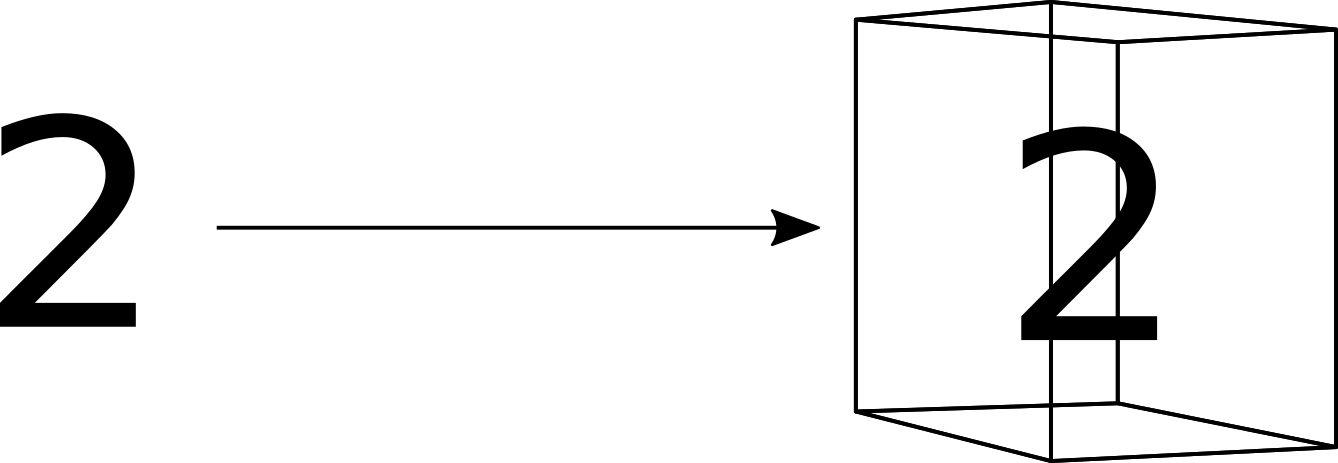
\includegraphics[width=\columnwidth]{return}\\
   \captionof{figure}{The return}
   \label{fig:monadreturn}
   \bigskip
}

The box in figure~\ref{fig:monadreturn} visualizes the monad and \verb\2\ is the value that is being put inside the monad.
With the return function any value can be put inside a monad.
When it is inside the monad it cannot be seen by the outside world.

This is where the bind comes in.

\subsubsection{The bind}
Having a monad is good, but what if you want to manipulate the value of the monad?
The \verb\>>=\ (pronounced \emph{bind}) function supplies this functionality~\cite{wadler1995monads}.

When we want to apply the function \verb\(+3)\ to the monad containing \verb\2\, we call bind.
Bind unpacks the monad, as visualised in figure~\ref{fig:monadbind1}.

{
   \bigskip
   \centering
   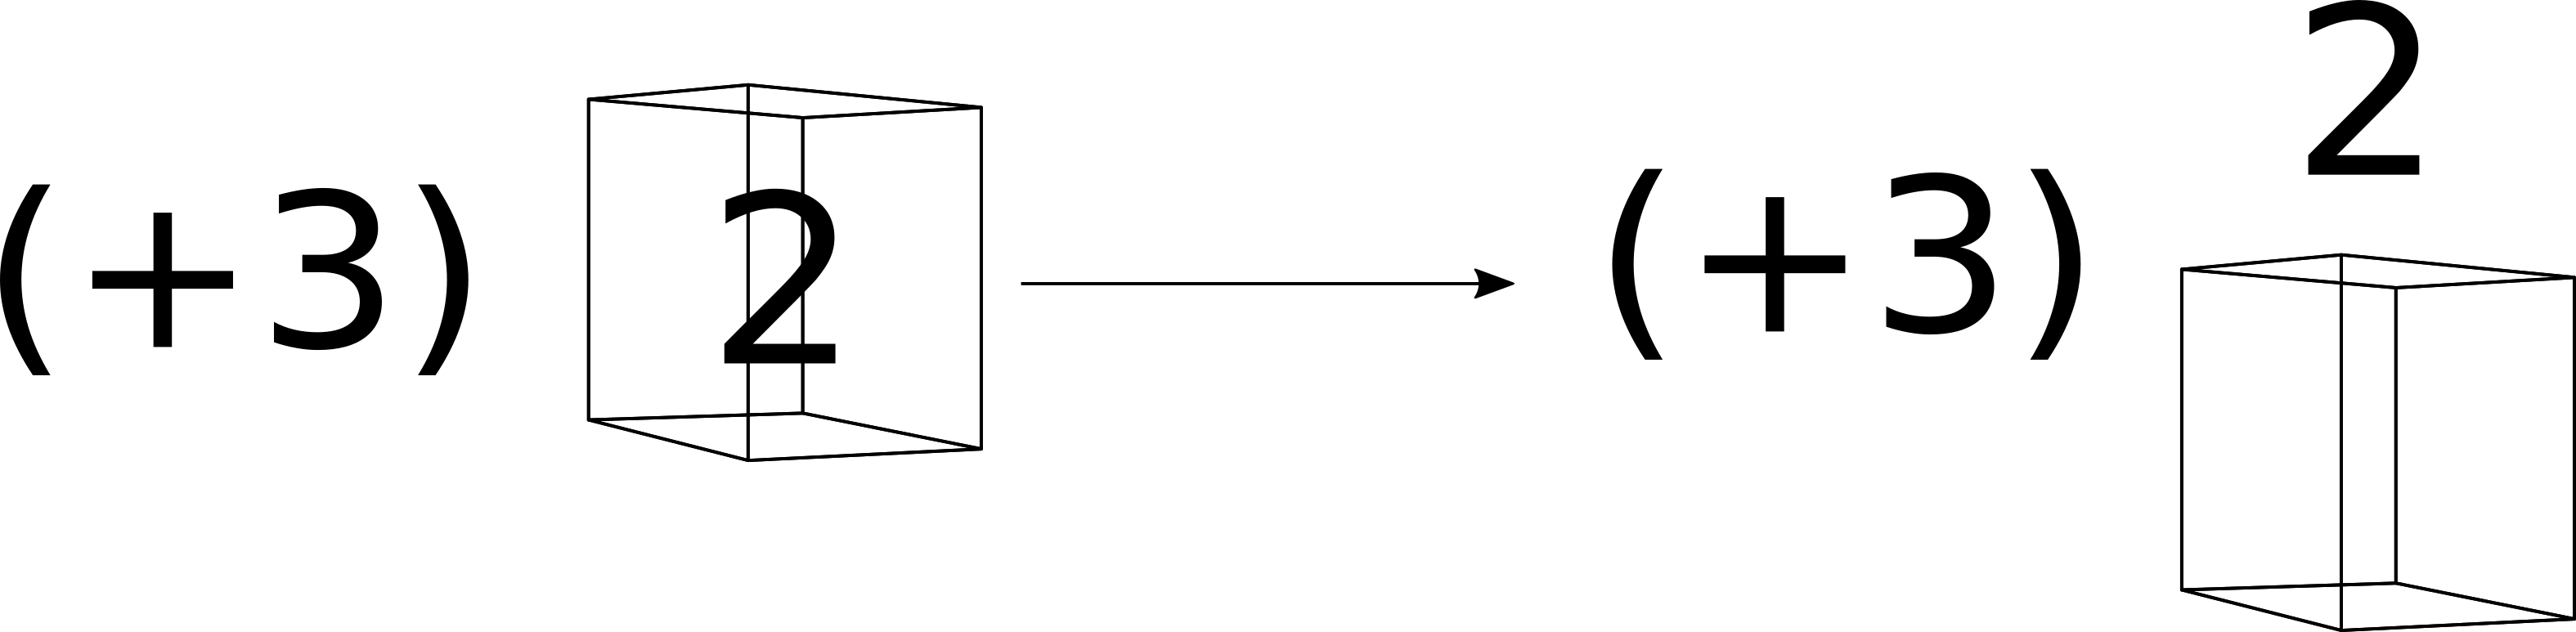
\includegraphics[width=\columnwidth]{bind1}\\
   \captionof{figure}{A function and a monad}
   \label{fig:monadbind1}
   \bigskip
}

It then applies the function to the value.
Finally the new value gets packed inside the monad by the function, as visualised in figure~\ref{fig:monadbind2}.

{
   \bigskip
   \centering
   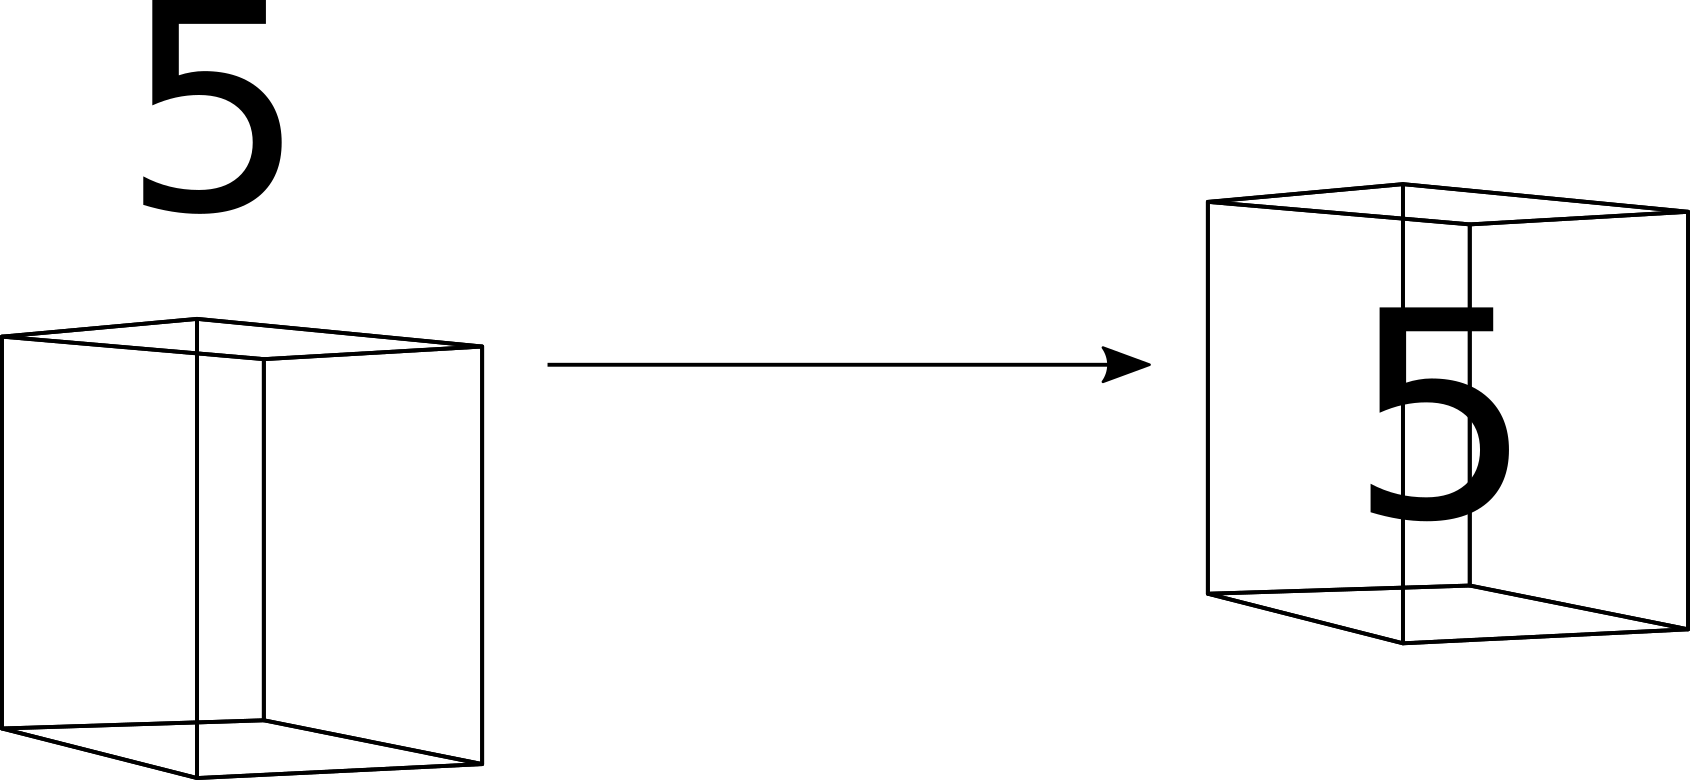
\includegraphics[width=\columnwidth]{bind2}\\
   \captionof{figure}{The return}
   \label{fig:monadbind2}
   \bigskip
}

Using these two basic functions, we can always work with monads and the values they contain.

To use the monads further we will need a few more functions.
These functions are generic for all the monads and will be given an implementation.


\subsubsection{More than a wrapper}
But just a monad offers very little besides being a wrapper for values.
That is why there have been created different sorts of monads.
This means a lot of different functionalities can be mapped to monads~\cite{moggi1991notions}.

We will discuss two of these for now.
More will be explained when looking at the implemented monads in MC in section~\ref{sec:standardimplementedmonads}.

\paragraph{The maybe monad}
offers the ability of the value to be either a value or nothing~\cite{swierstra2008data}.
For example we could utilize the pipe operator for this:

\begin{lstlisting}
Data "Maybe" -> 'a -> 'a | Unit

Func "test" -> Maybe -> Boolean^System
(match a with
  (\ x -> True^builtin)
  (\ unit -> False^builtin)) -> res
-----------------------------------
test a -> res
\end{lstlisting}

Here we use \verb\Unit\ as the nothing and 'a as the value.
In the example the term a is checked for a being a value, the \verb\Left\, or being nothing, the \verb\Right\.

This is a very basic example of how the maybe works.
It acts like a pipe and can contain either a value, \verb\Left\, or nothing, \verb\Right\.


\paragraph{The state monad}
gives monads the ability to behave like mutables.
It takes a \emph{state} and returns a new state and a return value~\cite{swierstra2008data}.

Say we want a random number generator.
The state monad will simulate the \emph{state} of the number being generated.
The state monad is given a \emph{state} in the form of a number and from this it will compute the new state of the number and the random number generated.

In MC the functionality might look like this:

\begin{lstlisting}
Func "state" -> 's -> ('a,'s)
state number -> (randomGeneratedNumber,newNumber)
\end{lstlisting}

\bigskip

The implementations of these monads are far from complete, these examples simply show the functionality of these monads.

We will now look at how the monad is really implemented within MC.


\subsection{Implementation}\label{sec:basicmonadsimplementation}
Because monads need to be able to manipulate type information, it is a good example of what MC is useful for.

With this monad we will be able to create actual monads, this can be seen as the base module for monads.
First we take a look at the declaration:

\begin{lstlisting}
TypeFunc "Monad" => (Type => Type) => Module
\end{lstlisting}

Monads are implemented as modules.
This way we can put the return and bind functions inside a monad.

The first argument is a function on type level.
It represents the monad it uses to wrap the result in.

When looking at the implementation we see that a module is created with the return and the bind:

\begin{lstlisting}
Monad 'M => Module {
  ArrowFunc 'M 'a -> ">>=" -> ('a -> 'M 'b) -> 'M 'b   #> 10
  Func "return" -> 'a -> 'M 'a
\end{lstlisting}

The bind is declared with \verb\ArrowFunc\ and is called \verb\>>=\.
It takes a monad as its first argument and a function as its second argument.

The function creates the new monad which is then returned.

The return takes a value, \verb\'a\, and wraps it inside the monad, \verb\'M\.

Both bind and return are only declared and not defined, because they are different for every monad created.
When creating a new monad bind and return will need to be defined.

Now we will add functionality to make the monads more practical for the user when programming.


\subsubsection{Returnfrom}
Sometimes we want to directly pass the value inside the monad instead of wrapping it.
This is done with \verb\returnFrom\~\cite{swierstra2008data}.

\begin{lstlisting}
Func "returnFrom" -> 'a -> 'a
returnFrom a -> a
\end{lstlisting}

As we can see the identifier \verb\a\ is directly passed on.


\subsubsection{Lift}
Lift is used when a regular function, it takes a value and returns a value, needs to be executed over a monad~\cite{jaskelioff2008monatron}.
Lift unwraps the monad, executes the function with the value of the monad and then wraps the new value inside the monad.

An important difference with the bind, is that the function given to the lift does not pack the value in a monad.
The function passed to the bind does pack the value inside the monad.

\begin{lstlisting}
  Func "lift" -> ('a -> 'b ) -> 'M 'a -> 'M 'b
  {a >>= a'
     return f a'} -> res
  ----------------------
  lift f a -> res
\end{lstlisting}

Here we can see clearly that the lift repacks the value with \verb\return\.

The \verb\Lift\ can also be declared with functions which take two arguments.
It is then called \verb\Lift2\.

\verb\Lift2\ has to bind twice, once for each monad.

\begin{lstlisting}
  Func "lift2" -> ('a -> 'b -> 'c) -> 'M 'a -> 'M 'b -> 'M 'c
  {a >>= a'
     b >>= b'
       return f a' b'} -> res
  ---------------------------
  lift2 f a b -> res
\end{lstlisting}

This can be expanded to functions which take any number of arguments.

With these functions we have the complete interface of a monad.
Now we can use the module \verb\Monad\ to implement them.


\subsubsection{Combining monads}
Monads can also be combined~\cite{king1993combining}.
Since they have the same generic interface they can be combined into another generic interface.
These new monads can utilise the functionality of the all combined monads.

In this way the functionality of a monad can be extended~\cite{king1993combining}.
Combining monads can be seen as putting one monad inside another monad.

We will take the state and maybe monad and combine these into a parser monad.
A parser monad can parse through a piece of text and scan for certain elements~\cite{liang1995monad}.

The state monad will be used for the scanning functionality and the maybe monad will be used to determine of the element has been found.
The state monad returns the maybe monad as its result.
When the maybe monad has a value as result the parser monad stops.

Like normal monads, combined monads have to be built manually.
This is a very error prone process when combining more than two monads or when using more complex monads.

What we actually want is to write the monads once and combine them automatically.
This is where monad transformers come in.


\subsection{Monad transformers}
Monad transformers are a way to automatically combine monads~\cite{liang1995monad}.
Instead of simply having a monad which takes the arguments it needs, it also takes another monad as one of its arguments.
The monad given as argument is then used to process the other arguments given to the monad transformer.

MC has an implementation of the basic monad transformer with which all monad transformers and monads can be created.

For monad transformers to work a generic function is added which contains the signature of the monad wrapped inside the transformer.

\begin{lstlisting}
TypeFunc "MCons" -> Type
MCons -> 'M
\end{lstlisting}

The identifier \verb\'M\ is the monad given to the monad transformer.
\verb\MCons\ can be called when this monad is needed directly.


\subsubsection{LiftM}
There are of course functions that work specifically with the wrapped monad in a monad transformer.
For this \verb\liftM\ is created.

For this we have to use the bind and return of the wrapped monad.
\begin{lstlisting}
  Func "liftM" -> (MCons^'M 'a -> MCons^M' 'b) -> 'M (MCons^'M 'a) -> 'M (Mcons^'M 'b)
  {M >>=^'M a
    f a -> b
    return^'M b} -> res
  ---------------------
  liftM f M -> res
}
\end{lstlisting}

It works the same as the other lift functions, with the specification of using the bind and return of the wrapped monad, \verb\'M\, instead of the bind and return of the current monad.


\subsection{Evolution of monad}
Monad was first implemented with just \verb\MCons\, \verb\>>=\, \verb\return\ and \verb\returnFrom\ functions.
This enabled basic use of the monad.

\verb\lift\, \verb\lift2\ and \verb\liftM\ were then added to extend the usecases of monads.


\section{Tryable monad}\label{sec:standardtryablemonad}
Apart from the regular monadic module there is also the tryable monadic module.
The tryable monad has as extra functionality that a function can be attempted.

This means that we can have functions that fail, without breaking the program.

It uses the regular monadic module to create a new interface.
It also takes a monad as an argument which it then inherits.

\begin{lstlisting}
TypeFunc "TryableMonad" => (Type => Type) => Module
TryableMonad 'M => Monad(MCons^'M) {
  inherit 'M
\end{lstlisting}

It uses the type signature of \verb\'M\ to create a new monad.

Here we see how \verb\MCons\ is used to get the signature of the original monad.

Then we declare the \verb\try\ function.
It takes a monad and two functions.

\begin{lstlisting}
  Func "try" => MCons^'M 'a => ('a -> MCons^'M 'b) => ('e -> MCons^'M 'b) => MCons^'M 'b
\end{lstlisting}

The value inside the monad is checked and then one of the functions is executed.
This will be done in the definition.

First the value inside the monad is put into a \verb\match\.

\begin{lstlisting}
  {pm >>=^'M x
    (match x with
\end{lstlisting}

If \verb\x\ contains an error the error function processes it.
And if it contains a value the value is passed to the function.

\begin{lstlisting}
      (\e -> err e)
      (\y -> k y)) -> z
\end{lstlisting}

The result of \verb\match\ is then wrapped in monad \verb\'M\ and returned.

\begin{lstlisting}
    return^'M z} -> res
  ---------------------
  try pm k err -> res
}
\end{lstlisting}

With \verb\try\ we can now check if the monad contains a value or an error and process them.

The \verb\try\ function was put to the test by manually typechecking it.
The resulting proof can be found in appendix~\ref{app:typeproofs}.

We also want to be able to get the original monad out of the tryable monad.
This is done with \verb\getMonad\.

\begin{lstlisting}
  TypeFunc "getMonad" => Type
  getMonad => MCons^'M
}
\end{lstlisting}

Now we can create a \verb\Monad\ which has two options when calling bind.
This can be used for error handling or for creating complex dataflows within monads.


\subsection{Evolution of tryable monad}
The \verb\TryableMonad\ started out as the \verb\either\ monad.
\verb\either\ used the available options to create error handling.

It occured then that we could also create more complex dataflows, when creating a generic tryable monad.
This was then implemented as the \verb\TryableMonad\.


\section{Implemented monads}\label{sec:standardimplementedmonads}
We will now look at the monads that are implemented in MC.

\subsection{Id}\label{sec:basicmonadsimplementedid}
If monad transformers always take another monad, there has to be at least one monad to end the chain.
That is where the \emph{id} monad comes in~\cite{liang1995monad}.

It does not take a monad as part of its arguments and simply returns all values as they are.

First we need a type signature to tell the monad interface which monad we are creating.

\begin{lstlisting}
TypeAlias "Id" => Type => Type
Id 'a => 'a
\end{lstlisting}

Here we can see what the id monad should do, simply pass the type on as it was given.

Now we will declare and define the id monad.
The type signature is created with \verb\Id\ and bind and return are defined.

\begin{lstlisting}
TypeFunc "id" => Monad
id => Monad(Id) {
  bind x k -> k x
  return x -> x
}
\end{lstlisting}

\verb\Id\ also takes an \verb\'a\, but this is never used as the id monad does not need an extra type to say which type it really uses.
While the \verb\'a\ is not used, it necessary to have them in the type signature.
Otherwise \verb\Id\ cannot be used to instantiate \verb\Monad\, as evident from section~\ref{sec:basicmonadsimplementation}.

Other monad transformers which do actually use the \verb\'a\ also do not instantiate them immediately.
The programmer can decide for which type the monads will be created, therefor it is left open.
This effectively creates an interface for the defined monad to be instantiated with a type later specified.

\verb\return\ simply returns the exact same value and \verb\bind\ executes the function \verb\k\ with \verb\x\ as its argument.
It is the monad which \emph{passes through} the values.

When using the \verb\id\ monad transformer with another transformer, it becomes that monad.

As an example we pass the \verb\id\ monad to the \verb\maybe\ monad transformer.
When the return of the created \verb\maybe\ monad is called, it first calls the return of the inner monad.
In this case is the \verb\id\ monad.

The return of the \verb\id\ monad returns the value directly as a result.
This result is then passed back to the \verb\maybe\ monad, where it gets wrapped inside the maybe monad and returned.

In this way the \verb\id\ monad will always end the cycle.


\subsection{List}\label{sec:standardmonadlist}
The \verb\list\ monad uses a list to store the values~\cite{king1993combining,swierstra2008data}.

The \verb\list\ monad transformer uses \verb\List\ from \emph{prelude} to create the transformer.

First we have to declare and define the signature.

\begin{lstlisting}
TypeAlias "ListT" => (Type => Type) => Type => Type
ListT 'M 'a => 'M(List 'a)
\end{lstlisting}

Using \verb\ListT\ together with the signature of \verb\'M\ we create the \verb\list\ monad.

\begin{lstlisting}
TypeFunc "list" => Monad => Monad
list 'M => Monad(ListT MCons^'M) {
\end{lstlisting}

\verb\ListT\ also takes a \verb\'a\, which is the type for the list created.
As stated in section~\ref{sec:basicmonadsimplementedid} the programmer has to decide which type the \verb\list\ monad uses.

The \verb\return\ simply puts the value in a one-element list wrapped inside a monad.

\begin{lstlisting}
  return x -> return^'M(x :: empty)
\end{lstlisting}

\verb\bind\ looks a bit more complicated.
It uses the \verb\ArrowFunc\ syntax together with a match.

\begin{lstlisting}
  {lm >>= l
    (match l with
\end{lstlisting}

The match checks whether the list is empty.

\begin{lstlisting}
      (\empty -> return^'M empty)
\end{lstlisting}

When a list is present the first element of the list gets unpacked by the bind of \verb\'M\, which gets named \verb\y\.
The function \verb\k\ gets executed with \verb\y\ as its argument and the result gets repacked by the return.

\begin{lstlisting}
      (\(x :: xs) ->
        {x >>=^'M y
          return^'M k y} -> z
\end{lstlisting}

Now the rest of the list, \verb\xs\, gets passed to the bind of \verb\list\ so the entire list gets passed to \verb\k\.
The results of processing \verb\x\ and \verb\xs\ are then concatenated into a single list.

\begin{lstlisting}
        xs >>= k -> zs
        (z @ zs)))} -> res
  -------------------------------
  lm >>= k -> res
}
\end{lstlisting}

All the nested functions are closed with the proper brackets and the resulting list is returned as the result of the bind.

If the use of the different syntaxes of the \verb\ArrowFunc\ seems confusing, take an extra look at section~\ref{sec:basicmcarrowfunc}.


\subsubsection{Evolution of list}
The list that is used within the list monad, was first implemented within the list monad.
But the list could be used outside of the monad as well.

It was then moved to \emph{prelude}.


\subsection{Either}\label{sec:basicmonadseither}
The \verb\either\ monad is an implementation of the \verb\TryableMonad\ module.

It creates a monad which can be either a value or a list of error messages~\cite{jaskelioff2008monatron}.
The type signature is as follows:

\begin{lstlisting}
TypeAlias "EitherT" => (Type => Type) => Type => Type => Type
EitherT 'M 'e 'a => 'M('a | 'e)
\end{lstlisting}

It uses the pipe to be able to be either failed or a value.
In the definition of \verb\either\, \verb\'e\ will be specified as a list.

The \verb\TryableMonad\ is then called with the signature of the monadic argument.

\begin{lstlisting}
TypeFunc "either" => Monad => Type => TryableMonad
either 'M 'e => TryableMonad(EitherT MCons^'M (List 'e)) {
\end{lstlisting}

The \verb\'a\ is again not used, like the id monad in section~\ref{sec:basicmonadsimplementedid}.

Next we have is the \verb\fail\ function.
It takes an error message and concatenates it with the existing error messages.

\begin{lstlisting}
  Func "fail" -> 'e -> MCons^'M
  fail e -> return^'M(Right (Right^'M :: e))
\end{lstlisting}

The \verb\fail\ is needed when we call the \verb\try\.
It will provide the error function to the \verb\try\.

Because \verb\either\ is a \verb\TryableMonad\ it can contain a value or an error message.
When calling the bind of \verb\either\ this needs to be checked.

That is why the bind calls \verb\try\.

\begin{lstlisting}
  pm >>= k -> try pm k fail
\end{lstlisting}

The monad and the function is passed on to \verb\try\ together with the function \verb\fail\.

The \verb\return\ passes the value to \verb\'M\.

\begin{lstlisting}
  return x -> return^'M(Left x)
\end{lstlisting}

\verb\Left\ is used because we know \verb\x\ is a value.


\subsubsection{Evolution of either}
\verb\either\ was first implemented without the use of \verb\TryableMonad\.
It had the same functionality.
All the functions of the \verb\TryableMonad\ were implemented directly within \verb\either\.

When the idea occurred of using a generic tryable monad, these were ported to the \verb\TryableMonad\.
\verb\either\ was then implemented by using the \verb\TryableMonad\.


\subsection{Result}
The result monad is a complete implementation of the either monad transformer from section~\ref{sec:basicmonadseither}.

The \verb\either\ monad still needs an error type and a type for the values it takes.
The result monad specifies the error type, leaving the type of the value for the programmer to specify.

Because all the functions in \verb\either\ are defined, result can directly call \verb\either\ with an error type.
No further function declarations or definitions are needed.

In the declaration we specify it returns a \verb\TryableMonad\, which \verb\either\ actually is.
In the definition we specify the error type to be \verb\String\.

\begin{lstlisting}
TypeFunc "result" => Monad => TryableMonad
result 'M => either MCons^'M (List String)
\end{lstlisting}

This creates an \verb\either\ with \verb\String\ as error type.


\subsubsection{Evolution of result}
The original idea of the \verb\result\ monad was a \verb\maybe\ monad with error handling in the form of a \verb\string\.

The \verb\result\ monad was first implemented in much the same way as the \verb\either\ monad, but with explicit use of \verb\String\ as the error handler.
When this was noticed, the \verb\result\ monad was implemented by using \verb\either\.


\subsection{State}
We have had a basic explanation of the state monad in section~\ref{sec:standardmonad} where we have seen that it is different from most monads.
The state monad does not acts like a lambda in monadic form.

Now we will see how the state monad transformer is implemented.
The type signature of the state monad transformer shows that it is a function.

\begin{lstlisting}
TypeAlias "StateT" => (Type => Type) => Type => Type => Type
StateT 'M 's 'a => ('s -> 'M('a * 's))
\end{lstlisting}

It takes a state and returns a monad containing a tuple of the resulting value and the new state.

We use \verb\StateT\ in the call to \verb\Monad\ so it knows what the type signature will be.

\begin{lstlisting}
TypeFunc "state" => Monad => Type => Monad
state 'M 's => Monad(StateT MCons^'M 's) {
\end{lstlisting}

When looking at return we see something new.
A lambda is created to match the type signature of the state monad.

\begin{lstlisting}
  return x -> (\ s -> return^'M(x,s))
\end{lstlisting}

\verb\x\ is set as the result of the state.

We see this happening also in the bind.
A lambda is created and in the function body of the lambda the computation happens.

\begin{lstlisting}
  (\ s ->
    {sm s >>=^'M x
      x -> (x',s')
      k x' s'}) -> res
  ---------------------
  sm >>= k -> res
\end{lstlisting}

Bind of \verb\'M\ is called and the result is then deconstructed to get to the tuple which it contains.
We know \verb\x\ is a tuple because it is the result from state monad \verb\sm\.
That \verb\x\ is a tuple, is evident by the type signature of the state monad.

The state monad also contains two extra functions.
They make it possible to get and set the state.

To get the state we call \verb\getState\.

\begin{lstlisting}
  Func "getState" -> MCons 's
  getState -> (\ s -> return^'M(s,s))
\end{lstlisting}

It sets the state as the result in the return lambda.
By defining return this way, you will get the state back when it is entered into the lambda.

To set the state we call \verb\setState\.

\begin{lstlisting}
  Func "setState" -> 's -> MCons Unit
  setState s -> (\ unit -> return^'M(unit,s))
}
\end{lstlisting}

It sets the result to unit and the state to the input state.


\section{Other monad implementations}
When comparing the monad transformers of MC with monad implementations of other languages, we quickly come to the conclusion that MC is very compact.

When looking at a monad implementation in Python\footnote{Appendix~\ref{app:monadspython}}, we see that the code for most monads is much longer.
And these are the direct implementations, not using monad transformers.

There are only few attempts made when it comes to monad transformers.
The main reason for this is the need for higher order types.

Haskell also has an implementation of monad transformers~\cite{haskelllibrary}, but these are far longer than the MC implementation.\footnote{See appendix~\ref{app:monadshaskell} for the source code of the state monad transformer.}

This shows what MC is capable of compared to most other languages.
With the use of higher order types the high abstractions used for monad transformers can be implemented with very little code.


\section{Advantages}
Now that we know what monads are and that MC has a clear implementation of them, we can look at the practical advantages.

We will focus on the video game industry, but the concepts are useful in other industries as well.

When programming with monads and monad transformers we can create a monad which does one function and combine it with other monads.
When combining monads more complex functionalities are created, but the way they are used does not change~\cite{liang1995monad,swierstra2008data}.

When the way of using monads does not change there is no need to comprehend how a specific monad does things.
We only need to know how to use it.

Monads then become very powerful black boxes~\cite{liang1995monad,wadler1995monads,swierstra2008data}.

For example we can create a networking monad which takes care of all the network communication.
We also create a graphical monad which takes care of filling the screen.
And as a final touch we create an input monad which takes care of all the user input.

When we combine these monads for video game development the only thing left to create is the game itself.

The video game developer can now focus on the video game itself, saving time on networking, user input and graphics.
When combining monads with the typesafety of MC, the video game developer has a significant advantage over his competitors.

Not only is the video game developer able to develop faster, the video game is also less prone to bugs.


